\documentclass[a4paper,twoside]{article}

\usepackage{epsfig}
\usepackage{subfigure}
\usepackage{calc}
\usepackage{amssymb}
\usepackage{amstext}
\usepackage{amsmath}
\usepackage{amsthm}
\usepackage{multicol,multirow, booktabs, todonotes}
\usepackage{pslatex}
\usepackage{apalike}
\usepackage{enumitem}
\usepackage{float}
%\usepackage[square,sort]{natbib}
\usepackage{SCITEPRESS}     % Please add other packages that you may need BEFORE the SCITEPRESS.sty package.

\subfigtopskip=0pt
\subfigcapskip=0pt
\subfigbottomskip=0pt

\begin{document}

\title{Overview of Usage Analytics on Cloud-based Applications}

\author{\authorname{Manoj Kesavulu, Duc-Tien Dang-Nguyen, Markus Helfert}
%\affiliation{Lero –-- Irish Software Research Organization}
\affiliation{School of Computing, Dublin City University, Dublin, Ireland}
\email{\{manoj.kesavulu, markus.helfert\}@lero.ie, duc-tien.dang-nguyen@dcu.ie}
}

\keywords{Usage Data, Data Extraction, Application Features, Functionality, Cloud, Software-as-a-Service (SaaS), User Behaviour}

\abstract{Features or functionalities provided by cloud-based applications are accessed by users through various interfaces such as web browser, mobile app, and command line interface. Yet for monitoring cloud-based applications, software developers and researchers have focused on web browsers. Software updates are provided for such applications based on the data acquired from the cloud monitoring components but usage data of the cloud application features are difficult to extract in a cloud environment as the usage data is spread across the interfaces on the front-end and the back-end. In this paper, we focus on the usage of the cloud application features from the user perspective and how to extract these data in a cloud environment. We define six criteria for the user-level usage data, analyse the existing usage data extraction techniques and propose a usage data extraction framework adhering to the defined criteria.}

\onecolumn \maketitle \normalsize \vfill

\section{\uppercase{Introduction}}
\label{sec:1 introduction}

\noindent Software monitoring is a well-matured field where applications post-deployment are monitored for their usage data to understand how the applications are used by end-users \cite{Pachidi2014UnderstandingMining}. The usage data is generated after the applications are deployed and being used in real-time by the end-users. This usage data deems necessary for software developers and architects to provide updates for the applications. The majority of the research in the software monitoring domain focus on collecting software operational data, event logs, resource usage monitoring in order to identify performance issues, errors and other usability problems \cite{Fabijan2015CustomerReview}. 

On the other hand, web usage mining field has seen a lot of development \cite{Gasparetti2016ModelingActivities,Ghezzi2014MiningApplications}. However, many lessons can be learned when compared to a cloud-based application, the cloud application can also be accessed by a smart-phone for example. Hence, usage data also lies in this device and the methods and techniques for analysing web usage by website visitors has significant differences, compared to how mobile applications are used by the user to access the cloud-based applications. The techniques that are used in web usage mining (and other related domains) need to be revised if they are intended for mining usage data in a cloud environment.

Cloud-based software applications deployed over the Internet offer various advantages over traditional software such as reduced time to benefit, scalability, access through various interfaces and so on. One of the main advantage of using cloud applications is the option to an end-user to access the cloud application using multiple devices (interfaces). So, it is critical for any usage monitoring component to consider all these interfaces as usage data sources. In this paper, we focus on usage data extraction in Software-as-a-Service (SaaS) layer of the cloud. We aim to create a framework that can be used to extract the usage data that is generated in the cloud system along with the interfaces used by the end-user to access the cloud system. This will help to understand the features that are important for the user and critical to the system. For example, the user might use a feature very rarely but it might still be critical to him/her such as an on-line bill payment feature where the user might use it once a month but still is a critical feature for him/her. This cannot be determined by analysing the frequency of usage of the feature by the user. Analysing and understanding the usage data from the users’ perspective can be used by the software developers and software architects to determine how much development time, development cost to allocate and spend for which features of the cloud application before rolling out new updates. As a part of our future work, we aim to build the usage data extraction artefact and follow the evaluation approach using Design Science Research \cite{Helfert2012TheFramework}.

The remainder of this paper has the following structure: We provide background on SaaS development lifecycle and usage data in the cloud in Section \ref{sec:2 background}. In Section \ref{sec:3 User-level usage data criteria}, we discuss the criteria that we have identified and provide justification while analysing the literature based on the criteria. In Section \ref{sec:4 usage data extraction framework}, we propose the usage data extraction framework that adheres to the criteria discussed in the previous section. Then in Section \ref{sec:5 conclusion and future work}, we provide the conclusion and show direction for the future work.

\section{\uppercase{Background}}
\label{sec:2 background}
\subsection{SaaS Software Development}
\label{subsec:2.1 SaaS Software Development}
\noindent Traditional IT (Information Technology) aligns resources according to the way the applications are deployed within dedicated infrastructure and data storage to fulfil business requirements. Cloud computing has emerged as a computing paradigm with benefits such as high scalability, reduced IT costs, on demand self-service, pay-as-you-go price models, elasticity in provision computing resources.

Cloud computing architecture defines three distinct services layers as shown in Figure \ref{fig:fig1}:

\begin{figure}[!h]
  %\vspace{-0.2cm}
 \centering
 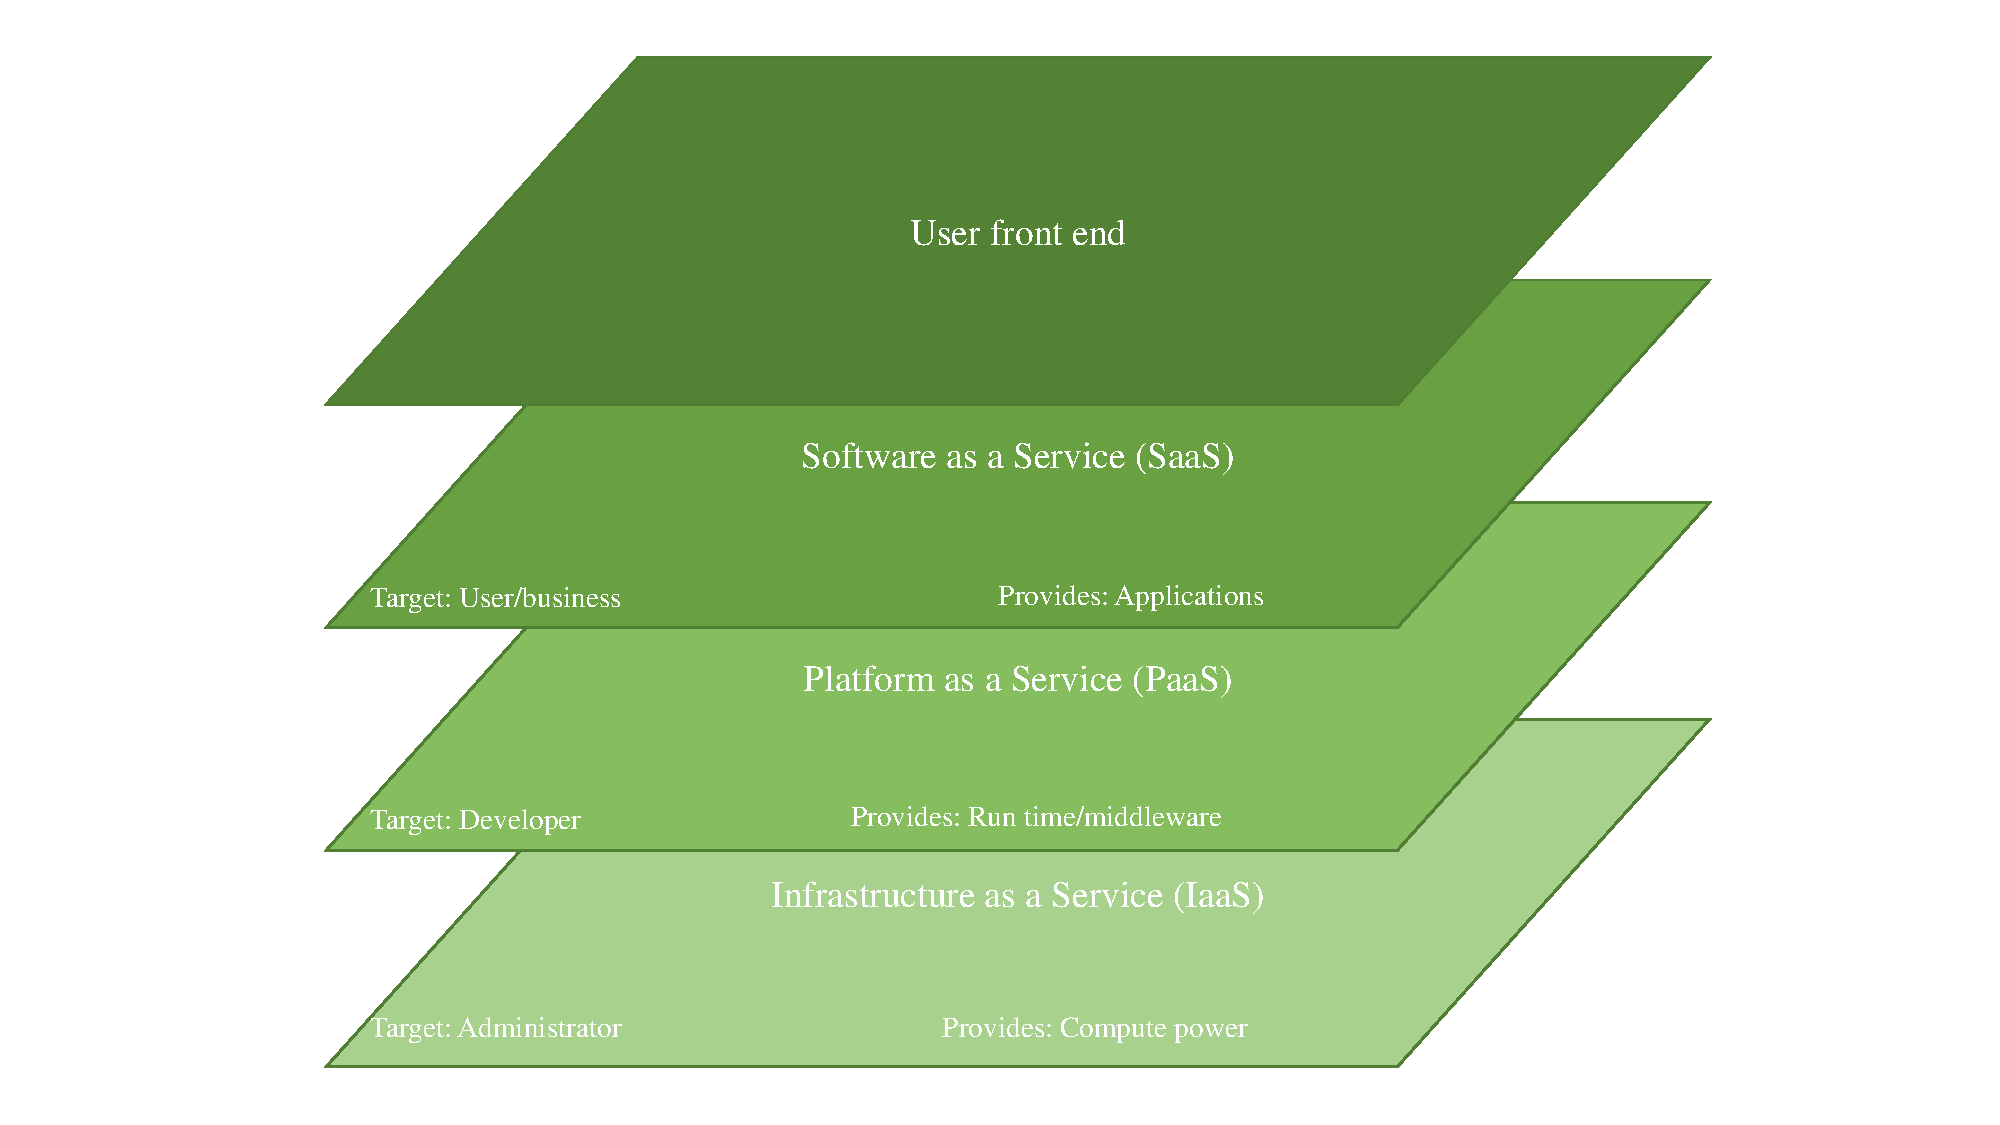
\includegraphics[width = 6cm]{Cloud_Service_Layers.pdf}
 \caption{Cloud Service Layers $[$Source: \cite{Pallis2010CloudComputing}$]$}
 \label{fig:fig1}
\end{figure}

The three distinct layers of the cloud are as follows:
\begin{itemize}
\item Infrastructure as a Service (IaaS) offers computing resources, both physical and virtual, for processing and storage.
\item Platform as a Service (PaaS) offers development environment for software developers to write their applications on a particular platform without worrying about the underlying hardware infrastructure.
\item Software as a Service (SaaS) offers software applications that can be accessed and used by the end-users.
\end{itemize}

The focus of our research is to understand what features and functionalities are important to the end-user by analyzing the end-user usage of the applications deployed in a cloud environment. We consider SaaS layer of the cloud where the user uses various interfaces to access the cloud-based applications. The widely-adopted definition for SaaS cloud model is provided by National Institute of Standards and Technology (NIST) as “The capability provided to the consumer is to use the provider’s applications running on a cloud infrastructure. The applications are accessible from various client devices through either a thin client interface, such as a web browser (e.g., web-based email), or a program interface” \cite{Mell2011TheComputing}. In other words, SaaS applications are deployed on cloud infrastructure and are provided to end-users as a service over the Internet, the end-users can access these applications using various interfaces such as web browsers, mobile applications and command line interfaces. These applications are often monitored by Application Performance Monitoring (APM) tools to understand how much of the underlying resources are used by the application, errors, bugs, usability issues and to identify outdated services where architectural refactoring can be applied while migrations applications to the cloud \cite{Kesavulu2017GenericPaper}. These data will be analysed by the application developers to fix the errors and bugs, improve the application and rollout updates. This constitutes the software development cycle in a SaaS environment as shown in Figure \ref{fig:fig2}. The software vendors are also interested in their customer behaviour to understand how end-users use the application. For this purpose, user behaviour knowledge is collected from analysing the user’s interaction with the web-browser while accessing the application in the form of clickstreams \cite{Pachidi2014UnderstandingMining,Wang2016UnsupervisedAnalysis}.

\begin{figure}[!h]
 %\hspace{-2cm}
 \centering
 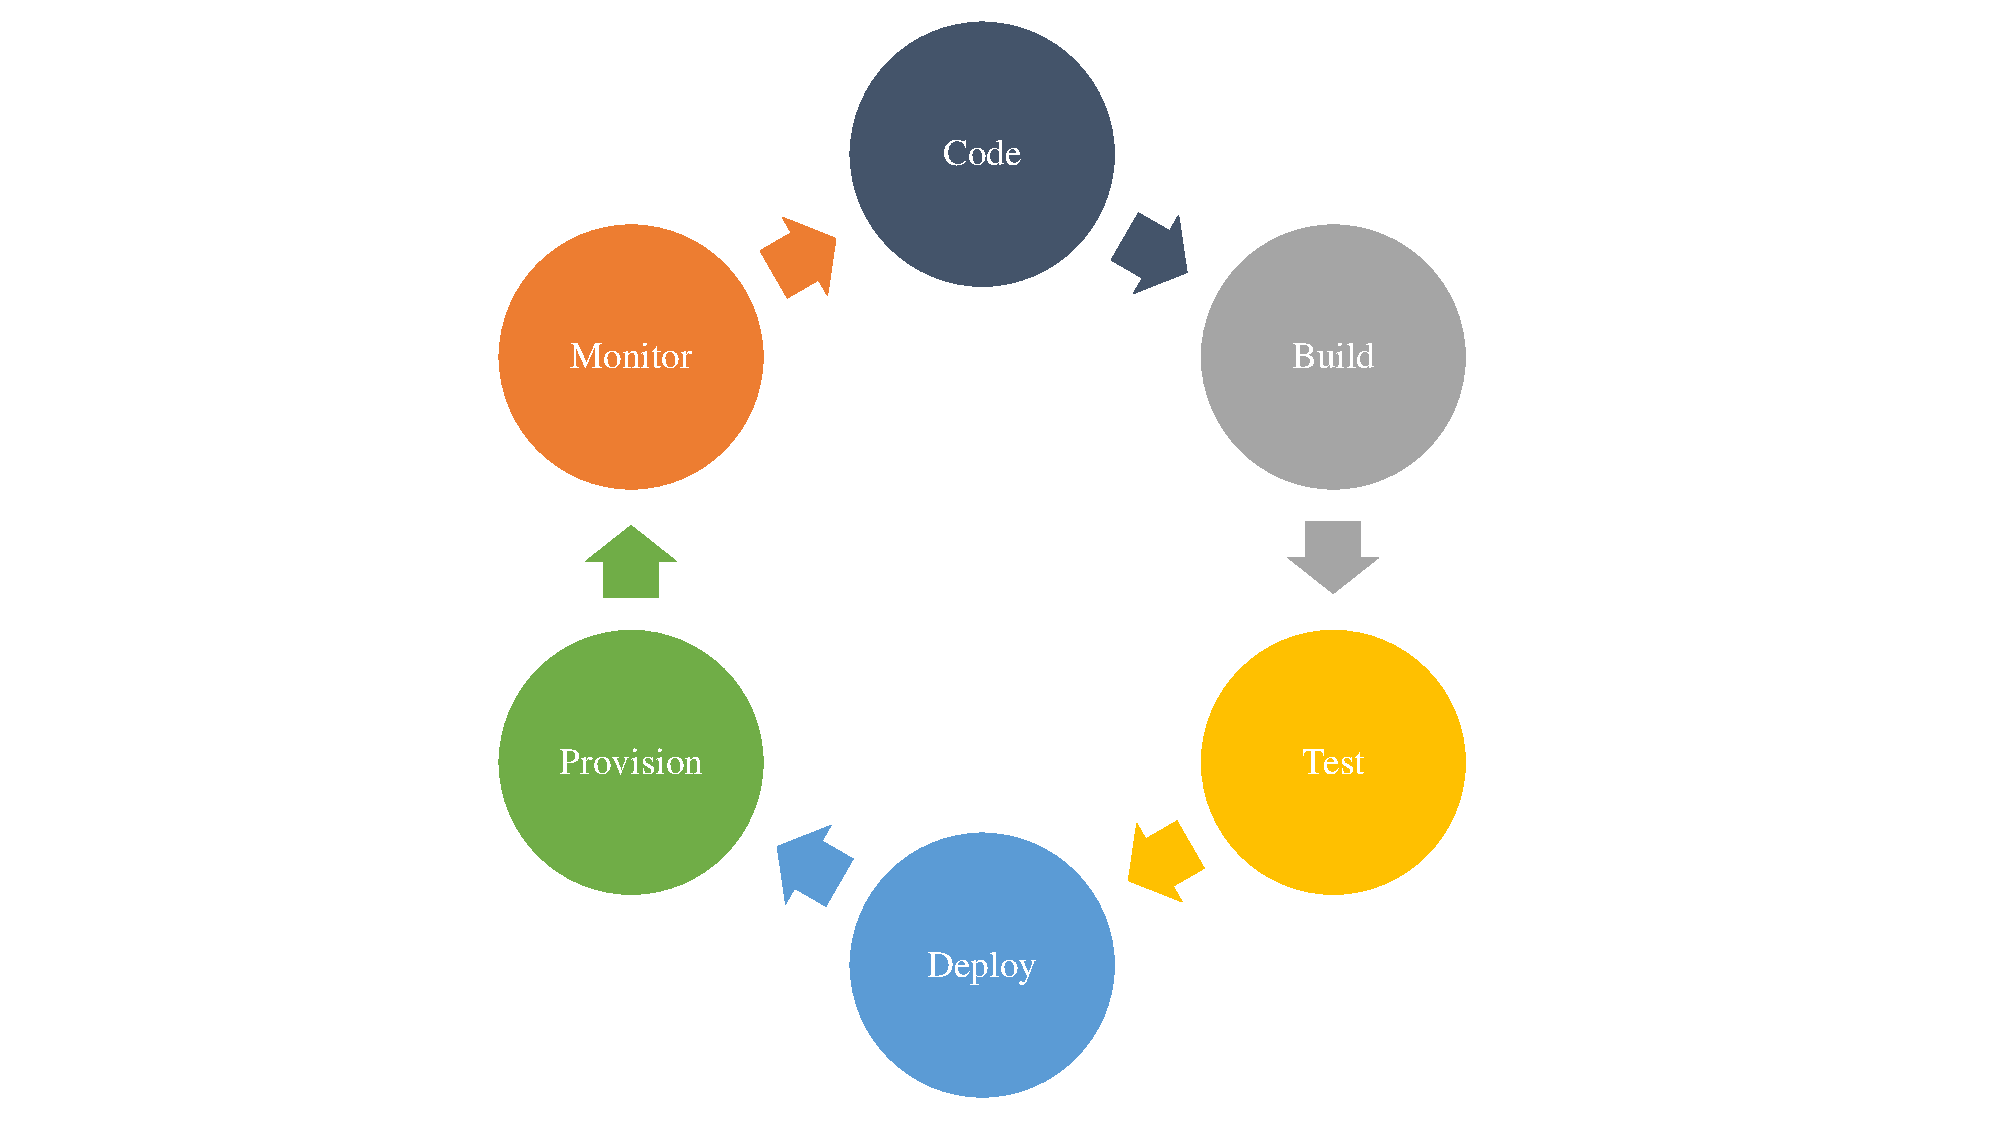
\includegraphics[width = 7cm]{SaaS_Software_Development_Lifecycle.pdf}
 \caption{SaaS Software Development Lifecycle}
 \label{fig:fig2}
\end{figure}

\subsection{Usage Data in Cloud}
\label{subsec:2.2 Usage Data in Cloud}

\noindent The rise of cloud computing and SaaS has eased the process of monitoring application usage as the applications are deployed on the cloud environment and provisioned to the end-user over the Internet as services. The cloud provider (vendor) provides APM tools (for example, CloudWatch (http://aws.amazon.com/cloudwatch/) in Amazon Web Services) to monitor the status of the deployed applications, the amount of resources used by the applications based on the agreement between cloud vendor and the application provider called Service Level Agreement (SLA). The application developers can also use various third-party monitoring tools such as New Relic (https://newrelic.com/), Binadox (https://www.binadox.com/salesforce-saas-monitoring/) and so on. But these tools mainly focus on monitoring application oriented usage such as measuring the number of users logged-in to the application, identifying rare logins, cloud resource usage, idle times, license types etc. Log files are analysed to derive models \cite{Petruch2012DerivingSimulations}. Understanding usage data of an application has various uses such as to personalise the application according to the end-users’ preferences \cite{Yang2017MultimediaPlatform}, profiling users for security \cite{Al-Bayati2016AdaptiveAnalysis}, improvement in marketing of software products \cite{Bucklin2009ClickMarketing} and to analyse the performance of the application in the deployed environment for maintenance purposes \cite{Petruch2012DerivingSimulations,Zaidman2010Multi-TenantPaper}.

From the literature exploration, we see that the idea of monitoring user behaviour is to understand how users interact with the application and this is mainly done through analysing the clickstreams \cite{Pachidi2014UnderstandingMining,Wang2016UnsupervisedAnalysis,Banerjee2001ClickstreamSubsequences,Bucklin2009ClickMarketing}. The authors \cite{Cito2015RuntimeFeedback} provide a high-level taxonomy of types of operation data: 

\begin{enumerate}
\item Monitoring data (Operational application metadata, Collected from state-of-the-art APM tools)
	\begin{enumerate}
		\item Performance data – service response times, database query times
        \item Load data – incoming request rate, server utilization
        \item Costs data – hourly cloud virtual machine costs, data transfer costs per 10,000 page views
        \item User behaviour data - clickstreams
	\end{enumerate}
\item Production data
	\begin{enumerate}
	\item Data produced by SaaS application itself-placed orders, customer information
	\end{enumerate}
\end{enumerate}

Consideration of user behaviour data only through clickstreams is mainly under the assumption that the end-user has access to the SaaS application only through a web-browser. Other interfaces such as mobile apps and command line interfaces are also used to access the application and these interfaces should be considered as sources for the extraction of the usage data from a cloud-based application.


\section{USER-LEVEL USAGE DATA CRITERIA}
\label{sec:3 User-level usage data criteria}

The user-level usage data in the context of this paper is the usage data generated because of user interaction with the SaaS application using which we can determine which features are critical and important for the end-user. Such data in the cloud is spread across various interfaces such as Web browser, mobile apps and command line interfaces on the front-end and server and database on the back-end. In order to classify the usage data, we refer the work from \cite{Pachidi2014UnderstandingMining} where the authors classify the usage data in a web-based system into six categories: (1) who is using the application; (2) Where the application being hosted; (3) What the end user does; (4) when the user performs the operation; (5) how long it takes to complete the operation; (6) other operation details such as errors, background tasks and number of records loaded. We add another category to this classification called user behaviour that contains clickstreams (from web-browser), view and focus (from mobile app) as a result of Human-Computer Interaction (HCI) between the end-user and the interfaces used to access the cloud-based application. The reason we refer to this classification is that SaaS applications are provisioned to the end-user over the Web and the rationale to add the new category (user behaviour) is because we focus on the usage data from the user perspective and the SaaS applications can be accessed through a mobile application in addition to a web-browser. We provide improved classification of the usage data as shown in Table \ref{table1}. \\

\begin{table}[!h]
\vspace{0.25cm}
\centering
\caption{Usage Data Classification $[$Adapted from \cite{Pachidi2014UnderstandingMining}$]$}
\begin{tabular}{l}
	\begin{tabular}[c]{@{}l@{}}1) Who is using the application\\ \quad a) User ID\\ \quad b) IP address\end{tabular}\\
\begin{tabular}[c]{@{}l@{}}2) Where the application is being hosted\\ \quad a) Web server\\ \quad b) Database\end{tabular}\\
\begin{tabular}[c]{@{}l@{}}3) What the end user does\\\quad a) Application\\\quad b) Page\\\quad c) Method \\\quad d) Function\\\quad e) Button that is accessed\\\quad f) Action that is performed\end{tabular} \\
\begin{tabular}[c]{@{}l@{}}4) When the user performs the operation\\\quad a) Date and time\\\quad b) Session ID\end{tabular}\\
\begin{tabular}[c]{@{}l@{}}5) How long it takes to complete the operation\\\quad a) Duration\\\quad b) Query duration\end{tabular}\\
\begin{tabular}[c]{@{}l@{}}6) Other operation details\\\quad a) Errors \\\quad b) Background tasks\\\quad c) Number of records loaded\end{tabular}\\
\begin{tabular}[c]{@{}l@{}}7) User behaviour\\\quad a) Clickstream\\\quad b) View\\\quad c) Focus\end{tabular}
\end{tabular}
\label{table1}
\vspace{0cm}
\end{table}

Some research is based on understanding user behaviour of smartphone users, where the users are grouped based on their smartphone application usage behaviour \cite{Zhao2016DiscoveringBehaviors}. The authors consider the recently used apps in the user’s smartphones and categorise the users into various types. But, the usage data is collected from an external source that is a Telecom company. These data is treated as biased and hence it is not reliable and not real-time. Though the authors provide a comprehensive explanation and detailed analysis steps on how the usage data was analysed to determine the user behaviour, since the usage data do not adhere to the criteria. It is uncertain whether their method applies to wide range of users globally. The authors in \cite{Cito2015RuntimeFeedback} aim at integrating runtime monitoring data from production deployments of the software into the development tools to enable tighter feedback loops. The authors call this notion as “Feedback-Driven Development (FDD)”. The authors argue that all the necessary data required is readily available in a cloud environment through built-in cloud monitoring APIs or through external APM solutions. Here, the authors purely rely on built-in or external tools to collect the data. But these tools consider only clickstreams for analysing the user behaviour. Since the end-users access the cloud applications through mobile apps and command line interfaces in addition to a web-browser, the usage data collected here may be treated as incomplete.

Considering the characteristics of the usage data to be extracted from a cloud system to understand the user behaviour, we propose six criteria for the usage data as follows: (1) Real-time –-- the usage data should be extracted while the user is interacting with the application; (2) Up-to-date --– the usage data should contain the recent data; (3) Complete --– usage data that is extracted should have no missing data; (4) Correct –-- the data extraction component should only collect relevant data i.e., only that data should be extracted that could represent the application features that are critical for the user; (5) Available –-- the usage data should be available to extract by the usage data extraction component; (6) Reliable –-- the data should be obtained from a reliable source i.e., unbiased.

Now that we have identified the criteria, we aim to analyse the existing usage data extraction and data analysis techniques according to the criteria, data collection procedure and the user interface(s) considered to collect the usage data as shown in Table \ref{table2}. Since the usage data is spread across front-end and back-end in a cloud environment and the front-end comprises of multiple interfaces for an end-user to access the SaaS application, we consider web-browser, mobile applications and command-line interfaces as the sources of usage data on the client-side. For this analysis, we started selecting the most recent papers on “monitoring SaaS application usage”. Since the selected papers refer to the older monitoring methods and techniques, we reached a saturation point and consideration of further older papers might not have yielded different results. 

As a result of the analysis, we see that completeness of usage data is seldom considered criteria and command line interface has been neglected as a source of usage data in front-end. The majority of the usage data extraction techniques and methods consider web-browser or mobile applications individually but not together. Since the SaaS applications can be used by the end-user through all the three interfaces, they should be considered as the usage data sources to understand the critical features of the application from the end-users’ perspective.

\begin{table*}[h]
	\centering
	\caption{Usage Data Extraction Framework Analysis}
	\label{table2}
	\begin{tabular}{|l|c|c|c|c|c|c|c|c|c|c|}
		\hline
		\multirow{2}{*}{\bf Papers} & \multicolumn{6}{|c|}{\bf Usage Data Criteria} & \multirow{2}{*}{\bf Data Collection Procedure} & \multicolumn{3}{|c|}{\bf User interface} \\
		\cmidrule{2-7}\cmidrule{9-11}
		& \rotatebox[origin=c]{90}{\bf Complete} & \rotatebox[origin=c]{90}{\bf Availability} & \rotatebox[origin=c]{90}{\bf Dynamic} & \rotatebox[origin=c]{90}{\bf Up-to-date} & \rotatebox[origin=c]{90}{\bf Reliable} & \rotatebox[origin=c]{90}{\bf Correct} &  & \rotatebox[origin=c]{90}{\bf Web browser} & \rotatebox[origin=c]{90}{\bf Mobile-App} & \rotatebox[origin=c]{90}{\bf CLI} \\
		\hline
		\cite{Pachidi2014UnderstandingMining} & & & X & X & X & & Code Injection & X & & \\
		\hline
		\cite{Zhao2016DiscoveringBehaviors}    & & & & X & & X & Manual (provided by a company) & & X & \\
		\hline
        \cite{Cito2015RuntimeFeedback} & & X & & X & X & & Cloud Monitoring Tools & X & & \\
		\hline
        \cite{Junco2013ComparingUse} & X & & X & X & X & X & 3\sup{rd} Party software & X & X & \\
		\hline
        \cite{Sarkar2014MiningReport} & & & & X & X & &  Internal Logging System & & & \\
		\hline
        \cite{Al-Bayati2016AdaptiveAnalysis} & & X & & & X & & Manual & & & \\
		\hline
        \cite{Xu2016LogFramework} & & X & X & X & X & X & Restful Interfaces & & & \\
		\hline
        \cite{Smit2013DistributedProcessing} & & & X & X & X & & Existing cloud monitoring tools & & & \\
		\hline
        \cite{Yang2017MultimediaPlatform} & & X & & & X & X & Application Plugins & & X & \\
		\hline
        \cite{Ghezzi2014MiningApplications} & & X & X & & X & X & URL Logging, REST & X & & \\
		\hline
        \cite{Yang2015CharacterizingInternet} & & & & X & & X & Manual (provided by a company) & & X & \\
		\hline
	\end{tabular}
\end{table*}

\section{USAGE DATA EXTRACTION FRAMEWORK}
\label{sec:4 usage data extraction framework}

\noindent This section describes the proposed framework called “Usage Data Extraction Framework”. It comprises different phases as shown in Figure \ref{fig:fig4}: Data Understanding, Data Classification, Data Sources Identification and Data Collection. The phases that are connected through the straight arrow are sequential, the dashed arrow represents the dependencies or outputs in each phase.


\emph{Data Understanding} refers to understanding what we need to know from the data we intend to extract from the cloud system. The usage data analysis may be useful for the analysis of user behaviour, application performance, software personalisation, recommendation, software development and so on. It is important to understand and decide what do we make of the usage data before continuing to the further phases.

\emph{Data Classification} refers to grouping the usage data as there exists various types of usage data and of various formats in a cloud environment. In this work, we classify the usage data into seven categories in a SaaS environment as shown in Table \ref{table1} in the data classification phase. 

\emph{Data Sources Identification} refers to the identification of the usage data sources. In this paper, we group the usage data sources into front-end and back-end, we emphasise on considering multiple user interfaces that end-users use to access the SaaS applications such as web browser, mobile applications and command-line interface as front-end usage data sources. Identifying these data sources is essential to understand the types and formats of the usage data, how the data is represented, stored and processed. 

\emph{Data Collection} refers to extraction of the usage data according to the classified types and identified formats. The usage data extracted should adhere to the proposed criteria: the data should be collected dynamically, that is, the usage data should the extracted while the user interacts with the SaaS application; complete - the usage data should be extracted from all the identified data sources; available – the usage data should be available at identified data sources; up-to-date – the usage data should have recent data from all the identified data sources; reliable – the data sources and the data extraction techniques and mechanisms should be reliable in nature and could be trusted, that is, the data extraction techniques should not tamper or manipulate the usage data during the extraction process; correct – the data extracted should be able to represent the purpose of the data as identified in the Data Understanding phase.

\begin{figure}[H]
%\vspace{-0.2cm}
 \centering
 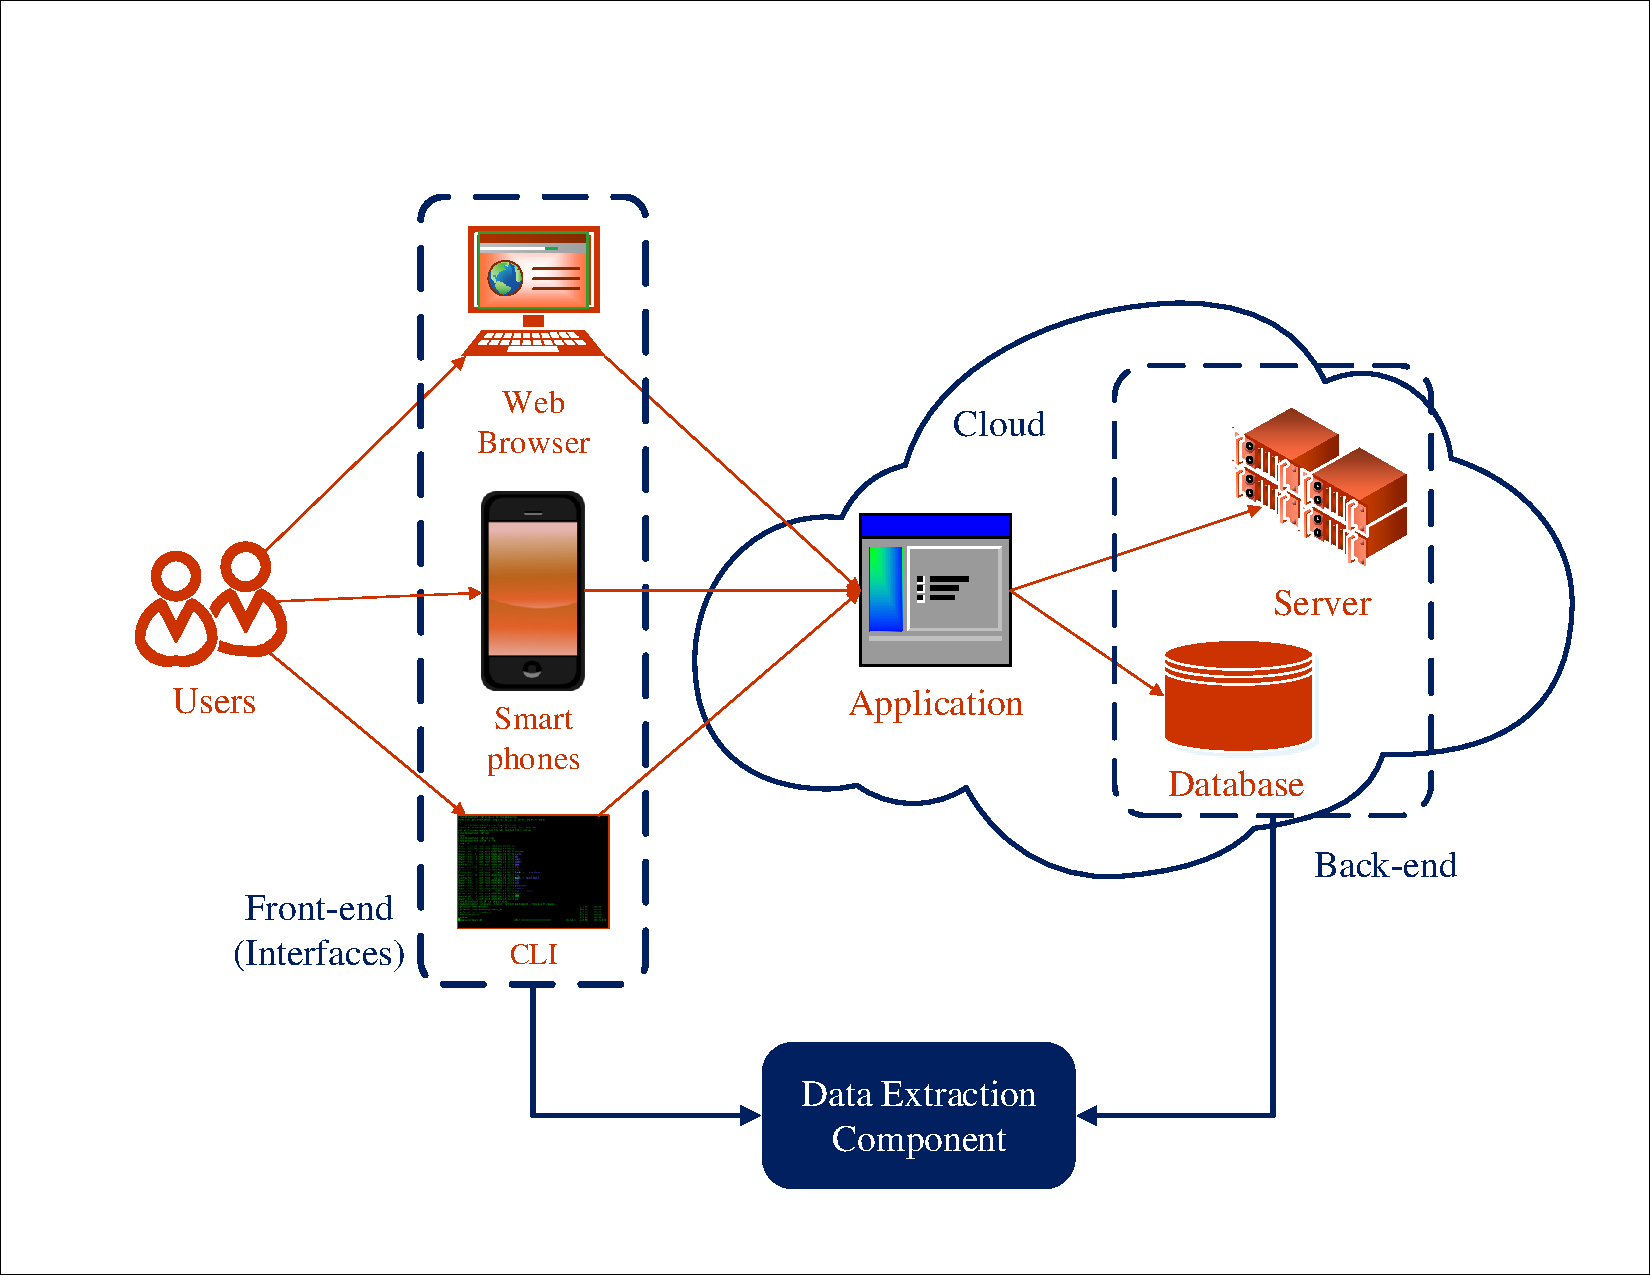
\includegraphics[width = 7.2cm]{SaaS_Data_Extraction.pdf}
 \caption{SaaS Usage Data Extraction}
 \label{fig:fig3}
\end{figure}

\begin{figure*}[h!]
  %\vspace{-0.2cm}
 \centering
 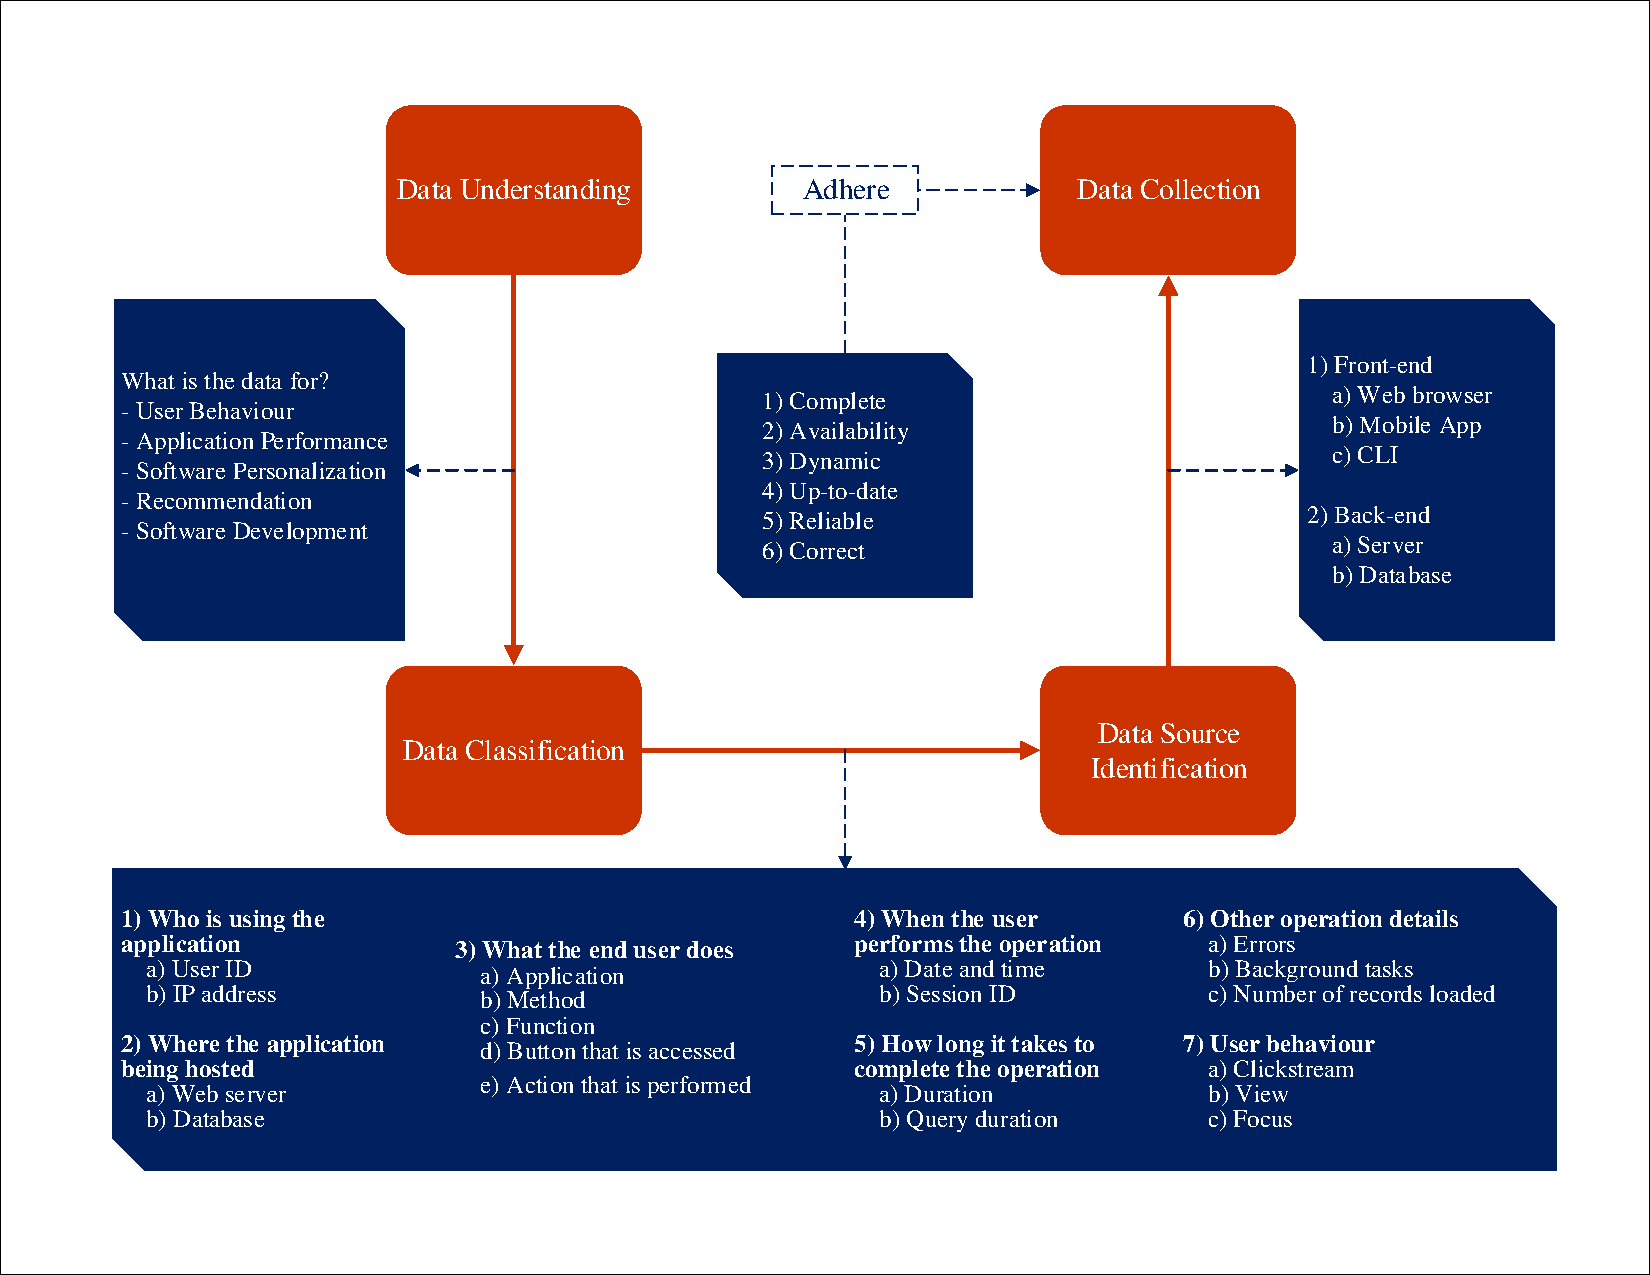
\includegraphics[width = 15.4cm]{Usage_Data_Extraction_Framework.pdf}
 \caption{Usage Data Extraction framework}
 \label{fig:fig4}
\end{figure*}

The framework we propose to extract usage data from a SaaS application considers web-browser, mobile application and command-line interface as usage data sources in front-end in addition to the back-end sources as shown in Figure \ref{fig:fig3}. Hence, satisfying the completeness criteria; since the sources of the usage data are the front-end and back-end of the SaaS application, the usage data extracted are available and reliable; the usage data is analysed to understand the purpose for the extraction of the usage data in the data understanding phase and classified according to various categories as shown in Table \ref{table1}, the usage data satisfies the correctness criteria. The data extraction component will be designed and developed in such a way that it extracts the usage data from the sources while the user interacts with the SaaS application, satisfying dynamic and up-to-date criteria. 


\subsection{Implementation Plan}
\label{subsec:4.1 Implementation Plan}
In this section we present a possible implementation of the framework. A SaaS application comprising a server and  database at the back-end and web-browser, smart-phone and command-line interface as interfaces to access this application at the front-end will be developed. Different types of users (U1, U2, U3 and so on) are created with different responsibilities. Various features (F1, F2, F3 and so on) of this application will be identified and each type of user is given access to use these features through the interfaces. According to the proposed framework, the first phase is to understand the purpose of extraction of the usage data. For the purpose of this project, we consider \emph{user behaviour, application performance, software personalization and software development}. The next phase is to classify the usage data into one of the seven types as shown in Table \ref{table1}, the classification of the usage data depends on the purpose identified in previous phase. Once the intended usage data to extract are identified and classified, the next step is to identify the data sources. A SaaS application can be accessed by an end-user through interfaces such as \emph{Web browser, Mobile App and Command-Line Interface} and the application is hosted on a \emph{Server} with the storage provided by a \emph{Database}. These 5 entities can be considered as the usage data sources. The final phase is \emph{Data Collection} phase, the extraction techniques used should adhere to the usage data criteria as discussed in Section \ref{sec:4 usage data extraction framework}. 


\subsection{Implications}
\label{subsec:4.2 implications}

The framework has many implications for different stakeholders of a SaaS application. This framework can be used by a software architect to design the usage data extraction or monitoring component for a SaaS based application while designing the application, the architect will first understand the intention or purpose of the usage data that the extraction component should extract. This understanding of the usage data will help in classifying the usage data types and the formats followed by different components of the cloud system. Using this classification, the architect can identify where the usage data resides in the cloud system and then can decide what methods and techniques should be used for the extraction. 

Data analyst can use this framework to better understand the nature of the usage data, the source of each data type, how the data is classified and extracted. Understanding the source of usage data and its classification could ease the analysis process. 
The software developer can use this usage data to understand the critical application features for an end-user, thereby prioritizing the features. This can improve the development time and cost for providing updates for the application.

The identified criteria for the usage data and the proposed usage data extraction framework can help researchers to consider and include all the interfaces used to access the cloud-based applications as usage data sources. This would lead to more replicable studies and results regarding development, instantiation and evaluation of the usage data extraction artefacts. 

\section{CONCLUSION AND FUTURE WORK}
\label{sec:5 conclusion and future work}

\noindent In this paper, we identified criteria for the usage data and analysed usage data extraction techniques according to the identified criteria, extraction procedure, and the considered user interfaces. We proposed usage data extraction framework with four phases: Data Understanding; Data classification --– we provide an improved usage data classification; Data Sources Identification –-- we identified that it is essential to consider mobile applications and command line interfaces as usage data sources in addition to the web-browser and Data collection. As a result of the criteria analysis, the main contribution of the paper is a novel usage data extraction framework as shown in Section \ref{sec:4 usage data extraction framework} which includes an improved usage data classification consisting of multiple interfaces as usage data sources on client-side for the purpose of usage data extraction, this framework includes all the usage data sources on the client-side such as web browser, mobile application and command-line interface. Hence, satisfying the ‘complete’ criteria of a usage data extraction component.

Our future work aims (i) to consider further the commercial usage data extraction solutions for analysis of the identified criteria, (ii) evaluate the framework using case studies, (iii) further improve the framework to include the usage data storage and analysis procedure (iv) design and development of usage data extraction artefact adhering to the proposed criteria and framework.

\section*{ACKNOWLEDGEMENT}
\noindent This work was supported with the financial support of the Science Foundation Ireland grant 13/RC/2094 and co-funded under the European Regional Development Fund through the Southern \& Eastern Regional Operational Programme to Lero - the Irish Software Research Centre (www.lero.ie)

\bibliographystyle{apalike}
{\small
\bibliography{Mendeley}}

\noindent----------------------------------------------------------
-----------------------------------------------------------



\vfill
\end{document}

